\documentclass[12pt]{article}
\usepackage{../lecture}
\lecture{16}{Directed Graphs, DAGs, and Topological Sort}
\date{March 23, 2021}

\begin{document}
\maketitle

\section{Directed Graph}
\begin{itemize}
    \item \textbf{Directed Graph} $G = (V, E)$: consist of a set of vertices/nodes $V$, and a set of edges/arcs $E \subseteq V \times V$.
    \item An edge is an ordered pair of vertices. $(u, v)$ is different from $(v, u)$.
\end{itemize}

\subsection{Directed Graph Representations}
\begin{itemize}
    \item Adjacency Matrix: $n \times n$ asymmetric matrix $A$. $A[u, v] = 1$ if $(u, v) \in E$ and $A[u, v] = 0$ if $(u, v) \notin E$. $A[u, v]$ is not the same as $A[v, u]$.
    \item Adjacency Lists: for each node $u$, $Out(u)$ (also referred to as $Adj(u)$) and $In(u)$ store out going edges and in coming edges from $u$. This is the default representation of a directed graph.
\end{itemize}

\subsection{Directed Connectivity}
\begin{itemize}
    \item \textbf{(Directed) Path}: a sequence of distinct vertices $v_1, v_2, ..., v_k$ such that $(v_i, v_{i + 1}) \in E$ for $1 \leq i \leq k - 1$. The length of the path is $k - 1$ and the path is from $v_1$ to $v_k$. By convention, a single node $u$ is a path of length $0$.
    \item \textbf{Reach}: a vertex $u$ can reach $v$ if there is a path from $u$ to $v$. $rch(u)$ is the set of all vertices reachable from $u$.
    \item \textbf{Asymmetricity}: a node $u$ can reach node $v$, but $v$ cannot reach $u$.
    \item \textbf{Strongly Connected}: $u$ is strongly connected to $v$ if $u$ can reach $v$, and $v$ can reach $u$. In other words, $v \in rch(u), u \in rch(v)$.
    \item Strongly connected is an equivalence relation, that is reflexive, symmetric, and transitive. The equivalence classes are strongly connected components, and they partition the vertices of $G$. $SCC(u)$ is the strongly connected component containing $u$.
\end{itemize}

\subsection{Directed Graph Connectivity Problems}
\begin{itemize}
    \item Given $G$ and nodes $u$ and $v$, can $u$ reach $v$?
    \item Given $G$ and $u$, compute $rch(u)$.
    \item Given $G$ and $u$, compute all $v$ that can reach $u$, that is all $v$ such that $u \in rch(v)$.
    \item Find the strongly connected component containing node $u$, that is $SCC(u)$.
    \item Is $G$ strongly connected (a single strong component)?
    \item Compute all strongly connected components of $G$.
\end{itemize}

\subsection{Basic Search in Directed Graphs}
\begin{itemize}
    \item Given $G = (V, E)$, a directed graph, and vertex $u \in V$. Let $n = \left| V \right|$.
    \item[] \lstinputlisting{code/basic-search-directed.sudo}
    \item \texttt{Explore(G, u)} terminates with $S = rch(u)$.
    \item $T$ is a search tree rooted at $u$ containing $S$ with edges directed away from root to leaves.
    \item Using \texttt{Explore(G, u)} to compute $rch(u)$ in $O(n + m)$ time, we can answer some connectivity problems.
    \begin{itemize}
        \item Given $G$ and nodes $u$ and $v$, can $u$ reach $v$?
        \item Given $G$ and $u$, compute $rch(u)$.
    \end{itemize}
    \item \textbf{Reverse Graph} $G^{rev}$: the graph with edge directions reversed, in other words $G^{rev} = (V, E')$ where $E' = \{ (y, x) \mid (x, y) \in E \}$.
    \item Computing $rch(u)$ on $G^{rev}$, we can answer some connectivity problems. This takes $O(m + n)$ time ($O(m + n)$ for $G^{rev}$ and $O(m + n)$ for $rch(u)$ via basic search).
    \begin{itemize}
        \item Given $G$ and $u$, compute all $v$ that can reach $u$, that is all $v$ such that $u \in rch(v)$.
    \end{itemize}
    \item $SCC(G, u) = \{ v \mid u \text{ is strongly connected to } v \}$
    \item Using $SCC(G, u) = rch(G, u) \cap rch (G^{rev}, u)$, we can answer another question in $O(m + n)$ time.
    \begin{itemize}
        \item Find the strongly connected component containing node $u$, that is compute $SCC(G, u)$.
    \end{itemize}
    \item Check if $SCC(G, u) = V$ for an arbitrary vertex $u$.
    \begin{itemize}
        \item Is $G$ strongly connected?
    \end{itemize}
    \item[] \lstinputlisting{code/strongly-connected-component.sudo}
    \item The above snippet takes $O(n(n + m))$.
    \begin{itemize}
        \item Find all strongly connected components of $G$.
    \end{itemize}
    \item $G^{SCC}$ is created by collapsing every strong connected component to a single vertex.
    \item For a directed graph $G$, its meta-graph $G^{SCC}$ is a DAG.
    \item[] 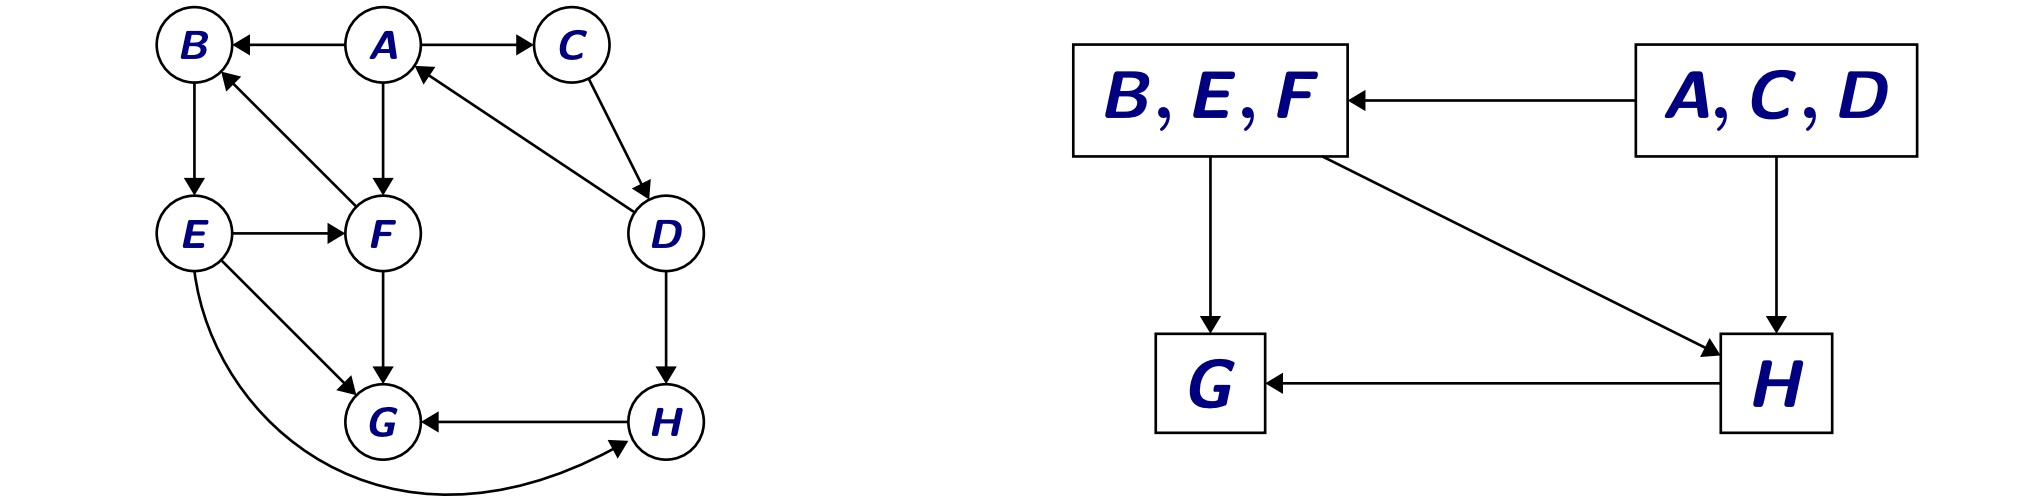
\includegraphics[width=\textwidth]{images/scc.jpg}
\end{itemize}

\section{Directed Acyclic Graphs}

\subsection{Simple DAG Properties}
\begin{itemize}
    \item \textbf{Directed Acyclic Graph}: A directed graph $G$ that has no directed cycle.
    \item \textbf{Source}: a vertex $u$ that has no incoming edges.
    \item \textbf{Sink}: a vertex $u$ that has no outgoing edges.
    \item Every DAG $G$ has atleast one source and atleast one sink.
    \begin{itemize}
        \item Let $P = v_1, v_2, ..., v_k$ be a longest path in $G$. Claim that $v_1$ is a source and $v_k$ is a sink.
        \item Suppose not. Then $v_1$ has an incoming edge which either creates a cycle or a longer path, both of which are contradictions. Similarly, if $v_k$ has an outgoing edge.
    \end{itemize}
    \item $G$ is a DAG if and only if $G^{rev}$ is a DAG.
    \item $G$ is a DAG if and only if each node is in its own strong connected component.
\end{itemize}

\subsection{Topological Ordering/Sorting}
\begin{itemize}
    \item \textbf{Topological Ordering/Sorting}: An ordering $\prec$ on $V$ such that if $(u, v) \in E$, then $u \prec v$.
    \item A DAG can be considered a dependency graph, and the topological ordering can be considered an order of events in which all dependencies are satisfied.
    \item A directed graph $G$ can be topologically ordered if and only if it is a DAG.
    \begin{itemize}
        \item A directed graph $G$ can be topologically ordered if it is a DAG.
        \begin{itemize}
            \item Pick a source $u$ and output it.
            \item Remove $u$ and all edges going out of $u$.
            \item Repeat until the graph is empty.
        \end{itemize}
        \item A directed graph $G$ can be topologically ordered only if it is a DAG.
        \begin{itemize}
            \item Suppose $G$ is not a DAG and has a topological ordering $\prec$. $G$ has a cycle $C = u_1, u_2, ..., u_k, u_1$.
            \item Then $u_1 \prec u_2 \prec ... \prec u_k \prec u_1$.
            \item That is $u_1 \prec u_1$.
            \item This is a contradiction (due to $\prec$ being an order).
        \end{itemize}
    \end{itemize}
    \item A DAG $G$ may have multiple topological sorts.
\end{itemize}

\end{document} 
